\documentclass[12pt]{article}

\usepackage{sbc-template}
\usepackage{graphicx,url,setspace,subfig, float}
\usepackage[utf8]{inputenc}
\usepackage[brazil]{babel}

\sloppy

\title{MAC5753 -- Sistemas Operacionais -- 2s2020\\ EP3}

\author{Guilherme Werneck de Oliveira\inst{1}}

\address{Departamento de Ciência da Computação -- Universidade de São Paulo (USP)\\
  Rua do Matão, 1010 - CEP 05508-090 - São Paulo - SP}

\begin{document}

\maketitle

\begin{abstract}
	This report describes the development and measured results of experiments carried out with file systems. A simulator was developed based on the FAT (File Allocation Table) structure and operations for writing and reading directories and files. The implemented experiments considered the program execution time in different states of the simulated system. The results presented showed an increase in the execution time according to the increase of the file size for copy operations. They also showed that the execution time was constant for the removal operations, regardless of the size of files and states of the simulator.
\end{abstract}

\begin{resumo}
  Este relatório descreve o desenvolvimento e os resultados aferidos de experimentos realizados com sistemas de arquivos. Foi desenvolvido um simulador baseado na estrutura FAT (File Allocation Table) e operações de escrita e leitura de diretórios e arquivos. Os experimentos realizados consideraram o tempo de execução do programa em diferentes estados do sistema simulado. Os resultados apresentados mostraram um aumento do tempo de execução de acordo com o aumento do tamanho dos arquivos para operações de cópia. Também, mostraram que o tempo de execução foi constante para as operações de remoção, independentemente do tamanho dos arquivos e estados do simulador.
\end{resumo}


\section{Introdução}

Um sistema de arquivos, em computação, tem como principal objetivo controlar como os dados são armazenados e recuperados de um dispositivo de armazenamento, independentemente de sua forma física. Ele possibilita que o sistema operacional leia e/ou grave diversos tipos de arquivos em diferentes endereços no disco, de forma a otimizar seu espaço de uso.

Para \cite{tanenbaum:16}, os requisitos essenciais para o armazenamento de dados são:

\begin{itemize}
	\item Armazenar uma grande quantidade de informações;
	\item As informações devem ser persistidas ao término dos processos que as utilizam; e
	\item Múltiplos processos devem ser capazes de acessar as informações ao mesmo tempo.
\end{itemize}

Este trabalho descreve o desenvolvimento de um simulador de sistema de arquivos e os resultados de testes aplicados, com o principal objetivo de analisar a estrutura e as principais operações em sistemas de arquivos.

\section{Descrição do Problema} \label{sec:firstpage}

A tarefa solicitada neste terceiro exercício prático (EP3) da disciplina de Sistemas Operacionais do 2º semestre de 2020 solicita a implementação de um simulador de arquivos baseado na abordagem FAT com tamanho de 100MB de armazenamento e blocos de 4KB.

Além da implementação da estrutura de arquivos, o simulador deve suportar a interação das seguintes operações por meio de um \textit{prompt}:

\begin{itemize}
	\item mount;
	\item cp;
	\item mkdir;
	\item rmdir;
	\item cat;
	\item touch;
	\item rm;
	\item ls;
	\item find;
	\item df;
	\item umount;
	\item sai.
\end{itemize}

Todas as alterações realizadas no simulador deverão ser armazenadas e, ao iniciar o simulador posteriormente, ele deverá continuar do mesmo estado em que foi finalizado.

\section{Descrição da Solução}

O código-fonte e os resultados aferidos estão disponíveis em \url{github.com/werneckg/mestrado/tree/master/SO/EP3}. A implementação do código-fonte foi estruturada da seguinte forma:
\begin{itemize}
	\item ep3.h, arquivo contendo o cabeçalho das funções utilizadas pelo ep3;
	\item ep3.c, implementação das funções utilizadas pelo ep3;
	\item main-ep3.c, arquivo contendo a implementação da função principal do ep3.
\end{itemize}

\subsection{O Sistema de Arquivos}

Para a implementação do sistema de arquivos baseado na estrutura FAT, foram considerados os elementos presentes na Figura~\ref{fig:fat} \cite{tanenbaum:16}. Por questões práticas, houve um arredondamento nos números de blocos implementados. Por exemplo, a quantidade de blocos totais foi arredondada para cima, pois 100MB divididos por 4KB (4096 bytes) é 24414,0625.

\begin{figure}[H]
	\centering
	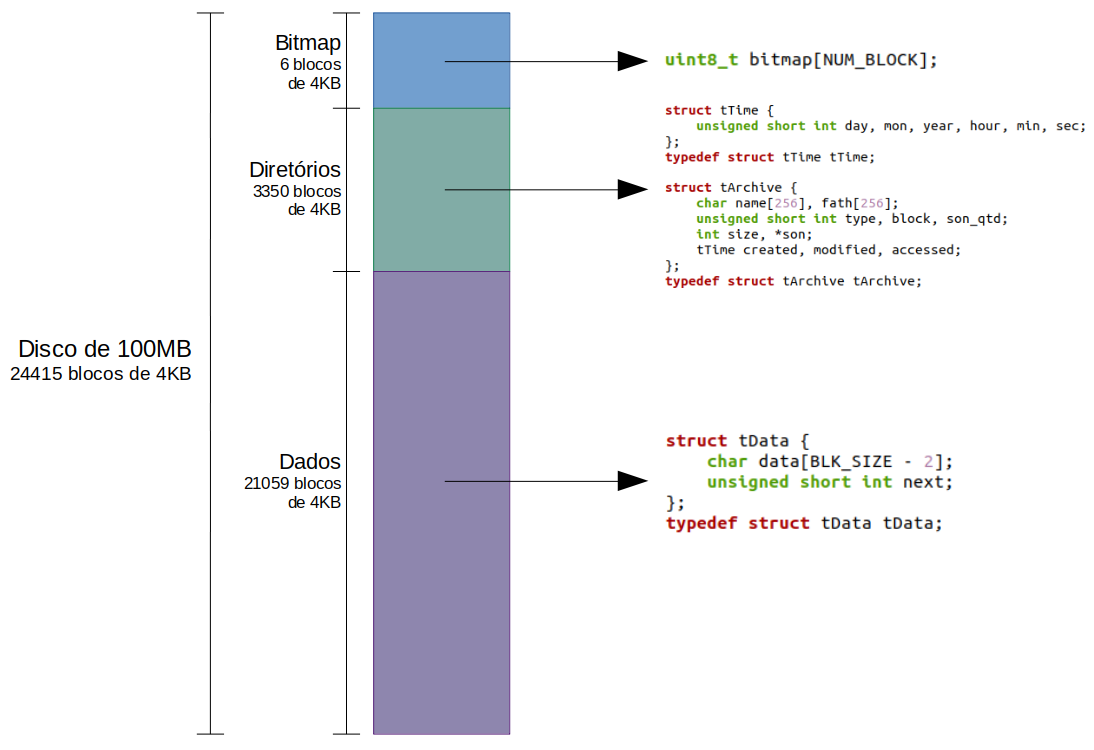
\includegraphics[width=1\textwidth]{fat.png}
	\caption{Representação da estrutura FAT implementada.}
	\label{fig:fat}
\end{figure}

O controle do espaço livre do sistema de aquivos implementado é realizado através do mapa de \textit{bits}, ou \textit{bitmap}, considerando o valor 0 como bloco ocupado e 1 como livre. Essa estrutura é representada por um vetor chamado \textit{bitmap}, como ilustrado na Figura~\ref{fig:fat}, de tamanho igual a quantidade de blocos do sistema.

Para a representação do registro dos metadados dos arquivos e diretórios, foi implementado um vetor do tipo \textit{tArchive} do tamanho do números de blocos menos a quantidade de blocos representada pelo \textit{bitmap}, uma vez que esse espaço é exclusivo para a gestão de espaço livre. A hierarquia de diretórios foi implementada por meio de um vetor dinâmico dentro da própria estrutura \textit{tArchive} onde cada entrada do vetor \textit{son} armazena a posição, no mesmo vetor de diretórios, do seu filho.

Já os blocos de dados são representados por um vetor de 21059 posições, pois 6 mais 3350 blocos já estão ocupados pelas estruturas do \textit{bitmap} e diretórios, respectivamente. Essa estrutura contém um vetor de caracteres e um tipo de dado inteiro utilizado para apontar o próximo bloco de dados caso o arquivo armazenado ocupe mais de um bloco.

\subsection{As Operações}

Todas as operações requisitadas na descrição do EP foram implementadas. Para que os comandos solicitados ao \textit{prompt} sejam executados, tanto os nomes dos diretórios quanto os dos arquivos devem ser escritos com o caminho completo, por exemplo, cat /$<$diretório$>$/$<$arquivo$>$. No caso em que o arquivo esteja no diretório ``/", o comando será cat /$<$arquivo$>$. As operações têm os seguintes comportamentos:

\begin{itemize}
	\item mount $<$arquivo$>$: monta o sistema de arquivos situado em $<$arquivo$>$. Esse comando considera o último estado do sistema em que o $<$arquivo$>$ foi utilizado. No caso em que o sistema não seja encontrado ele cria um novo contendo apenas o diretório raiz, ou seja, o ``/";
	\item cp $<$origem$>$ $<$destino$>$: copia o conteúdo do arquivo $<$origem$>$ hospedado no sistema de arquivos real do computador para o $<$destino$>$ no sistema de arquivos simulado;
	\item mkdir $<$diretório$>$: cria um novo diretório no sistema de arquivos simulado;
	\item rmdir $<$diretório$>$: remove um diretório existente no sistema de arquivos simulado e todo seu conteúdo;
	\item cat $<$arquivo$>$: mostra na tela o conteúdo do $<$arquivo$>$ caso ele exista no simulador;
	\item touch $<$arquivo$>$: atualiza o atributo de tempo de acesso do $<$arquivo$>$ caso ele exista no simulador. Caso ele não exista, um novo é criado com tamanho 0. Consequentemente, não há alocação de blocos de dados para ele;
	\item rm $<$arquivo$>$: remove o $<$arquivo$>$ do simulador;
	\item ls $<$diretório$>$: apresenta na tela o conteúdo do $<$diretório$>$, seja ele arquivos ou diretórios. Esse comando considera, também, o conteúdo de seus subdiretórios;
	\item find $<$diretório$>$ $<$arquivo$>$: busca no $<$diretório$>$ se há algum $<$arquivo$>$ e apresenta seu nome caso haja;
	\item df: apresenta a quantidade de diretórios, a quantidade de arquivos, o espaço livre e o espaço desperdiçado do sistema de aquivos simulado;
	\item umount: desmonta o sistema de arquivos simulado;
	\item sai: sai do simulador.
\end{itemize}

\section{Resultados Obtidos}

Para que os testes fossem realizados, foi implementado um módulo de testes juntamente com o simulador. Para maiores detalhes sobre sua execução, consultar o README disponibilizado com o código.

Os resultados apresentados foram obtidos a partir da execução do simulador de arquivos em uma máquina física com processador Intel® Core i5 com 4 CPUs, 6 GB de memória RAM e sistema operacional Ubuntu 20.04.1 LTS.

Os valores apresentados nos gráficos a seguir foram obtidos a partir de 30 execuções do simulador para cada um dos casos de teste e foram aferidos com um intervalo de 95\% de confiança. Os casos de teste executados foram:

\begin{itemize}
	\item Cópia de um arquivo de 1MB no ‘/’;
	\item Cópia de um arquivo de 10MB no ‘/’;
	\item Cópia de um arquivo de 30MB no ‘/’;
	\item Remoção de um arquivo de 1MB no ‘/’;
	\item Remoção de um arquivo de 10MB no ‘/’;
	\item Remoção de um arquivo de 30MB no ‘/’;
	\item Remoção completa de um diretório “pai” com 30 níveis de hierarquia abaixo dele e sem arquivo regular em nenhum dos subdiretórios;
	\item Remoção completa de um diretório “pai” com 30 níveis de hierarquia abaixo dele e com centenas de arquivos regulares em todos os subdiretórios.
\end{itemize}

Cada caso de teste foi executado considerando os seguintes estados do sistema de arquivos simulado:

\begin{itemize}
	\item Estado 1: Sistema de arquivos vazio;
	\item Estado 2: Sistema de arquivos com 10MB ocupados;
	\item Estado 3: Sistema de arquivos com 50MB ocupados.
\end{itemize}

A aferição do tempo de execução foi realizada com o uso da função \textit{clock()}, contida na biblioteca \textit{$<$time.h$>$}, imediatamente antes e depois da execução de cada caso de teste.

O gráfico ilustrado na Figura~\ref{fig:case1} apresenta o tempo de execução do simulador para o caso de teste referente à cópia de um arquivo de 1MB no sistema simulado nos três estados diferentes: sistema de arquivos vazio, com 10MB e 50MB ocupados. O primeiro fato observado foi o aumento do tempo de execução nos três diferentes estados. Esse aumento representou cerca de 13\% entre os estados 1 e 2. Já entre os estados 2 e 3 o aumento foi de aproximadamente 11\%. Isso se deve ao fato de que o simulador precisa encontrar um bloco vazio no vetor que representa o \textit{bitmap} e, quanto mais ocupado o sistema esteja, mais custosa se torna a busca. Esse fato também foi observado nos casos de teste ilustrados nas Figuras~\ref{fig:case2} e \ref{fig:case3}.

\begin{figure}[H]
	\centering
	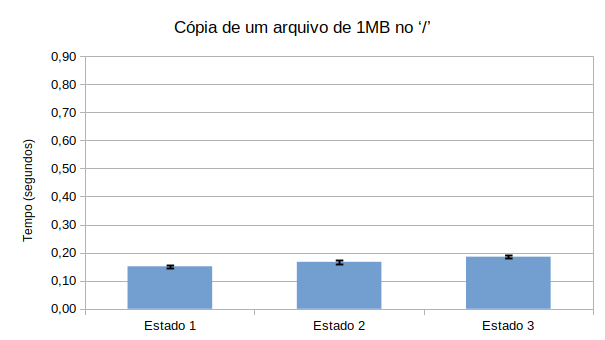
\includegraphics[width=1\textwidth]{case1.png}
	\caption{Tempo de execução do simulador para cópia de arquivo de 1MB.}
	\label{fig:case1}
\end{figure}

O aumento no tempo de execução nos três estados diferentes também foi observado nos casos de teste de cópia de um arquivos de 10MB e 30MB, Figuras~\ref{fig:case2} e \ref{fig:case3}. Esse aumento foi de 7\% e 23\% entre os estados 1 e 2 e 3 para cópia de 10MB, respectivamente. Para a cópia de 30MB, o aumento foi de 8\% entre os estados 1 e 2 e de 27\% entre os estados 2 e 3.

Quando comparados os valores entre os casos de teste de cópias de arquivos, o aumento foi de 86\% entre 1MB e 10MB para o estado 1. Para o estado 2, o aumento foi de 76\% e, para o estado 3, foi de 94\%. Para os casos de cópias entre 10MB e 30MB, o aumento representou 125\% para o estado 1, 126\% para o estado 2 e 135\% para o estado 3.

\begin{figure}[H]
	\centering
	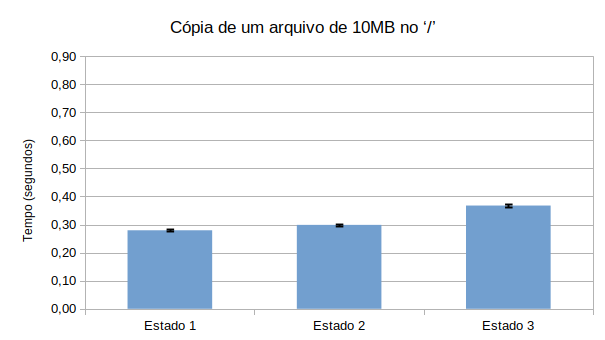
\includegraphics[width=1\textwidth]{case2.png}
	\caption{Tempo de execução do simulador para cópia de arquivo de 10MB.}
	\label{fig:case2}
\end{figure}

\begin{figure}[H]
	\centering
	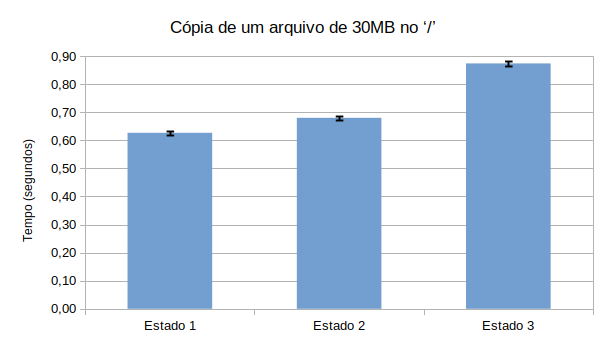
\includegraphics[width=1\textwidth]{case3.png}
	\caption{Tempo de execução do simulador para cópia de arquivo de 30MB.}
	\label{fig:case3}
\end{figure}

As Figuras~\ref{fig:case4}, \ref{fig:case5} e \ref{fig:case6} ilustram os resultados obtidos dos casos de teste referentes à remoção de arquivos do simulador. Foi observado que os valores aferidos foram constantes em todos os casos, tanto entre estados quanto entre os diferentes tamanhos de arquivos removidos. Esse comportamento era esperado, pois a operação de remoção de um arquivo, qualquer que seja seu tamanho ou até mesmo a quantidade ocupada no sistema de armazenamento, é realizada através de operações de liberação de espaço feitas no vetor do \textit{bitmap}.

\begin{figure}[H]
	\centering
	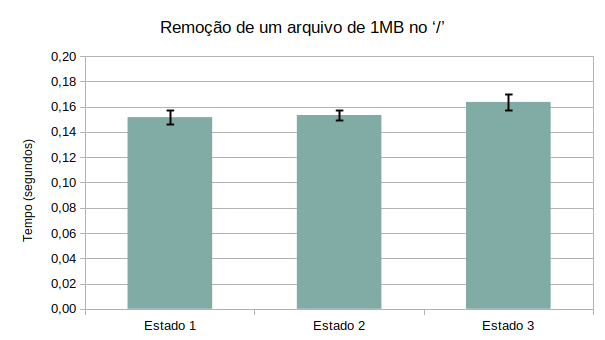
\includegraphics[width=1\textwidth]{case4.png}
	\caption{Tempo de execução do simulador para remoção de arquivo de 1MB.}
	\label{fig:case4}
\end{figure}

\begin{figure}[H]
	\centering
	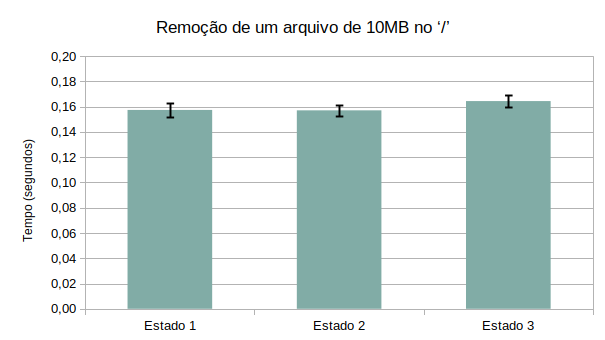
\includegraphics[width=1\textwidth]{case5.png}
	\caption{Tempo de execução do simulador para remoção de arquivo de 10MB.}
	\label{fig:case5}
\end{figure}

\begin{figure}[H]
	\centering
	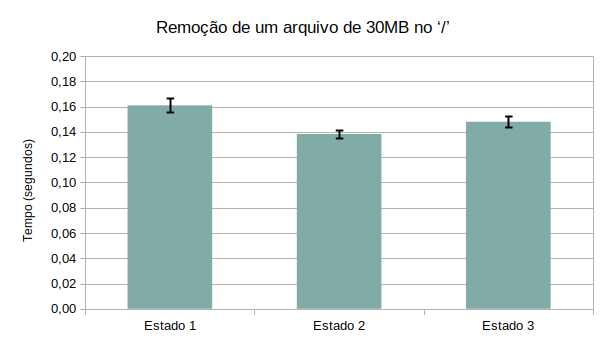
\includegraphics[width=1\textwidth]{case6.png}
	\caption{Tempo de execução do simulador para remoção de arquivo de 30MB.}
	\label{fig:case6}
\end{figure}

Por fim, as Figuras~\ref{fig:case7} e \ref{fig:case8} ilustram os valores obtidos para os casos de teste de remoção de diretórios que contêm subdiretórios e arquivos. Foi observado que o tempo de execução foi constante entre os estados. No entanto, houve um aumento de 100\% entre o primeiro e o segundo caso de remoção de diretórios em todos os diferentes estados. Isso se deve à mesma justificativa descrita anteriormente, relacionada à operação de liberação de espaço no vetor que representa o \textit{bitmap}.

\begin{figure}[H]
	\centering
	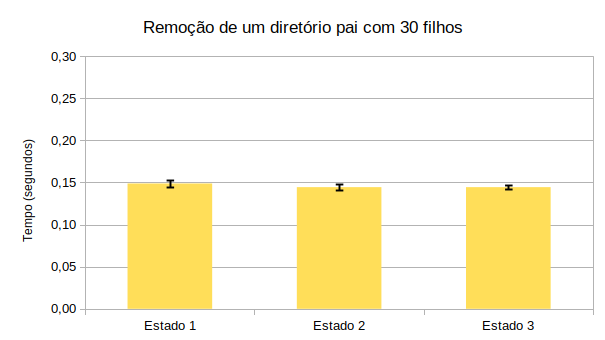
\includegraphics[width=1\textwidth]{case7.png}
	\caption{Tempo de execução do simulador para remoção de um diretório pai com 30 subdiretórios.}
	\label{fig:case7}
\end{figure}

\begin{figure}[H]
	\centering
	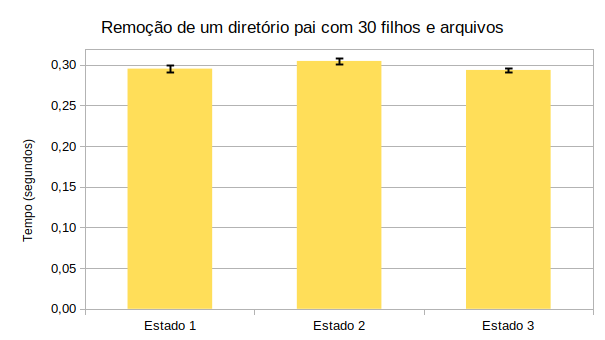
\includegraphics[width=1\textwidth]{case8.png}
	\caption{Tempo de execução do simulador para remoção de um diretório pai com 30 subdiretórios e arquivos.}
	\label{fig:case8}
\end{figure}


\bibliographystyle{sbc}
\bibliography{sbc-template}

\end{document}
